\chapter{Environment}
\label{chapter:environment}

Telecommunications computing ... The computing locates in various data centers as described in Figure \ref{fig:AirFrame}. Central data centers are built to massive warehouses that take advantage of centralized maintenance and 

Telco environment
Central data center vs far edge cloud in general

\begin{figure}[ht]
  \begin{center}
    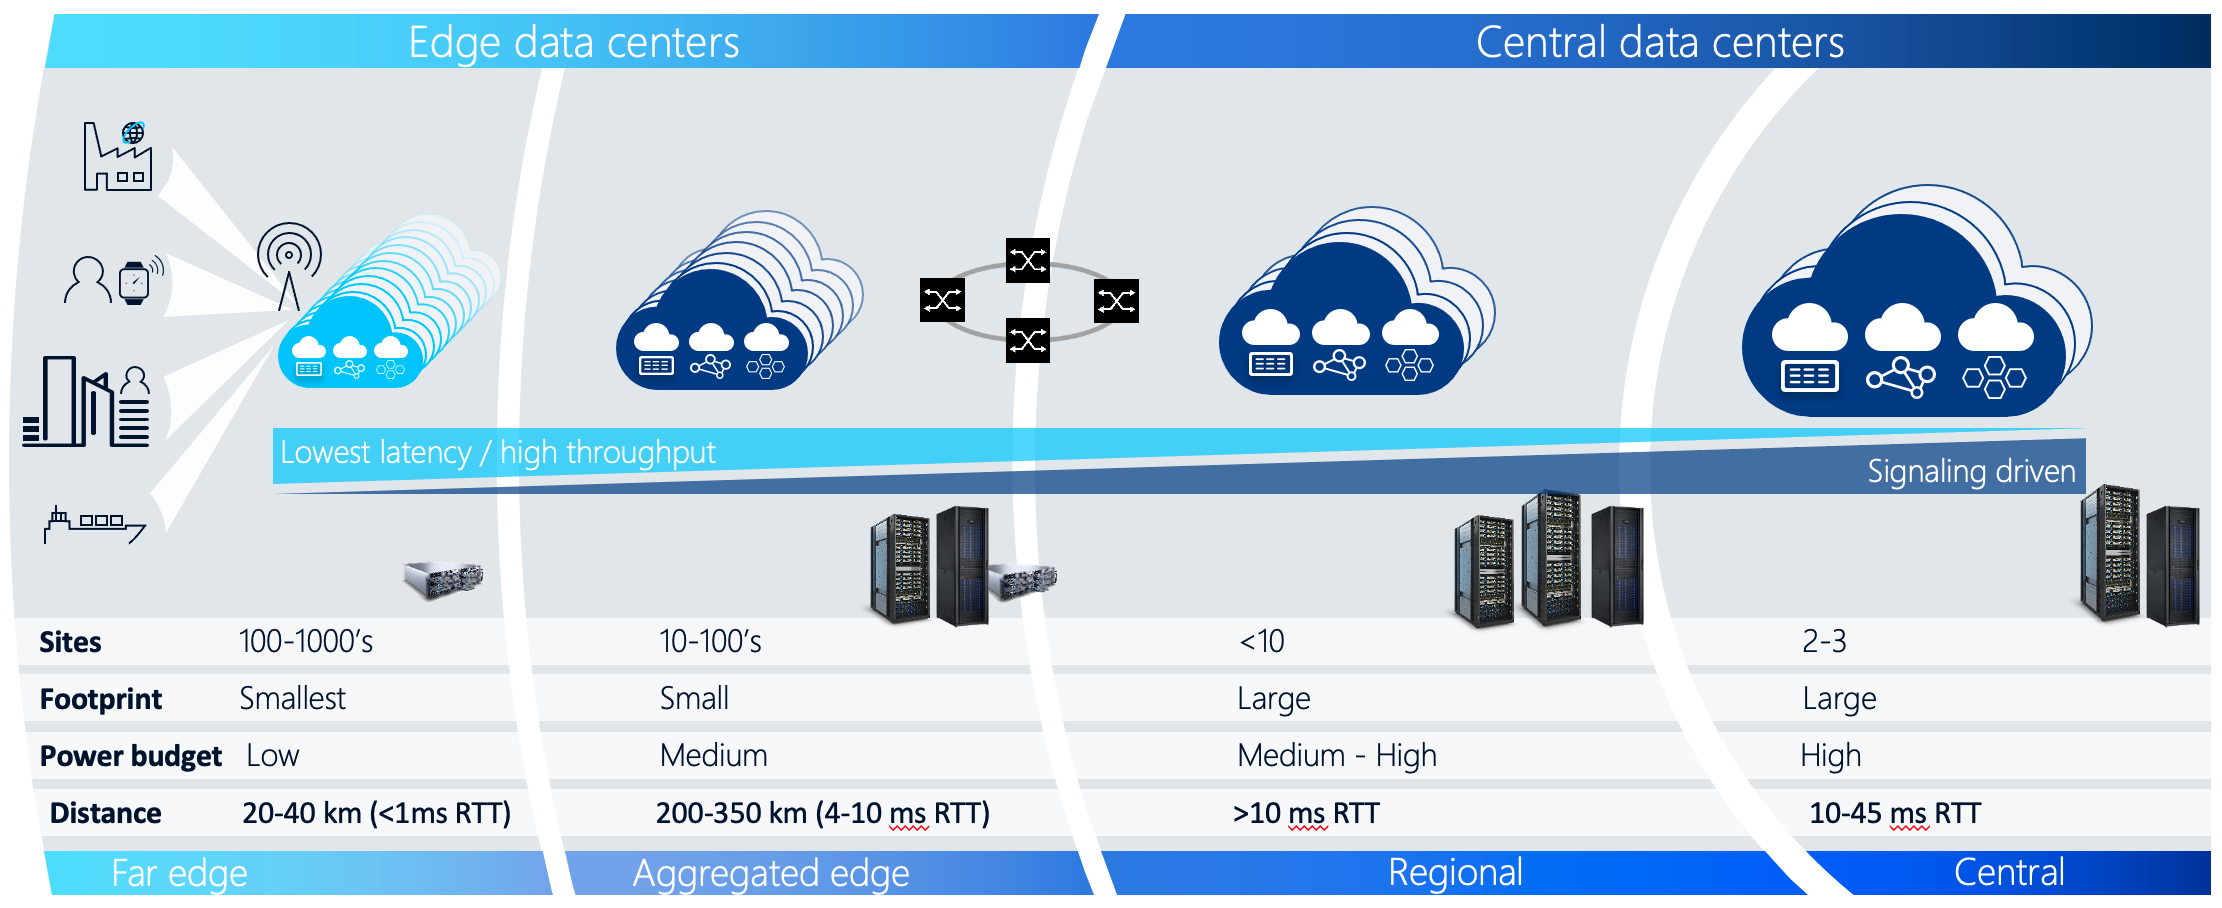
\includegraphics[width=13.5cm]{LaTeX/images/AirFrame.png}
    \caption{Far edge comparison to central data center \cite{AirFrameOpenEdgeServer}}
    \label{fig:AirFrame}
  \end{center}
\end{figure}

\section{Multi-access Edge Computing}

Multi-access Edge Computing (MEC) places compute and storage resources in the Radio Access Network (RAN) improving the delivery of content and applications to end user. MEC improves network efficiency by processing data on the mobile network cell instead of hauling it completely back to regional or central data centers for processing. The data can be processed partially or completely on the MEC node. For example, large public venues, such as stadiums or arenas, are good candidates for MEC, especially where localized venue services are important. In this use case, video created at a sports event or concert is served to on-site consumers from a MEC server, running appropriate applications located on the stadium premises. This video traffic is locally stored, processed and delivered directly to users at the event and does not require backhaul to a centralized core network and to then be returned to the user at the venue. The local processing of data reduces perceived latency on end-user and limits stress on the backhaul network. \cite{Brown2016}

Efficient capacity vs low latency & efficient transport

MEC covers two edge entities: aggregated edge and far edge. Aggregated edge locates usually at most 200 to 350 kilometers away from the end user and promises 4 to 10 millisecond round trip time (RTT).

\subsection{Far Edge Cloud}

Benefits of far edge
    - Latency
    - Allowing thin clients / offloading task to edge
    - Price and effect to environment
    - Security
    - Centralized repairing / upgrading (?)
    - Less power consumption
    - Flexibility in installment
    



\subsection{Applications}


\subsection{SR-IOV}
\label{section:SR-IOV}

I/O performance is critical to high performance telco systems. I/O intensive servers may waste CPU cycles, waiting for I/O data or spinning on idle cycles, which reduces system performance and increases latency. Single Root I/O Virtualization (SR-IOV) standard allows an I/O device, such as network interface controller (NIC), to be shared by multiple VMs. The SR-IOV technology is a hardware based virtualization solution that improves both performance and scalability. \cite{Dong2012}

Traditionally, when a guest accesses the I/O device, VMM needs to intervene in the data processing to share the physical device. The VMM intervention leads to additional I/O overhead for a guest OS. SR-IOV provides hardware enhancements for the Peripheral Component Interconnect Express (PCIe) device, which aims to remove major VMM intervention for performance data movement, such as the packet classification and address translation. An SR-IOV-capable device is able to create multiple light-weight instances of PCI function entities, known as Virtual Functions (VF). Each VF can be assigned to a VM for direct access, but still shares major device resources, achieving both resource sharing and high performance. \cite{Dong2012}





Requirements
- Root
- SR-IOV
- NICS

- Environment in MEC application
    - How migrated?
    - Elevated privileges and other requirements compared
    - Something else?
Nokia's environment \\
Usage of KC in Nokia's environment \\





% Comment: If your sentence ends in a capital letter write \@ before the period

% If you do need a normal space after a period (instead of
% the longer sentence separator), use \  (backslash and space) after the
% period. Like so: a.\ first item, b.\ second item.